\documentclass[10pt]{beamer}

\usepackage{cmap}%allows cyrillic search in pdf
\usepackage[english,russian,ukrainian]{babel}
\usepackage[T2A]{fontenc}
\usepackage[utf8]{inputenc}

\usetheme[progressbar=frametitle]{metropolis}
\usepackage{appendixnumberbeamer}

\usepackage{booktabs}
%\usepackage[scale=2]{ccicons}

%\usepackage{pgfplots}
%\usepgfplotslibrary{dateplot}

%\usepackage{xspace}
%\newcommand{\themename}{\textbf{\textsc{metropolis}}\xspace}

\usepackage{wrapfig,graphicx,caption,subcaption,overpic,tikz}
\usepackage{amsmath, amssymb, amsfonts}
\usepackage{tabularx, threeparttable, tablefootnote, multirow, multicol}
\usefonttheme[onlymath]{serif}
\usepackage{xcolor}

\title{ЕЛЕКТРОФІЗИЧНІ ВЛАСТИВОСТІ\\ БАГАТОФАЗНИХ ДИСПЕРСНИХ СИСТЕМ}
% \subtitle{A modern beamer theme}
% \date{\today}
\date{}

\author{
% \centering
\vspace{-10pt}
Семенов Андрій Костянтинович\\
Одеський національний університет імені І.І. Мечникова
% Дисертацiя на здобуття наукового ступеня\\
% кандидата фiзико-математичних наук
}

\institute{
{\bf Науковий керівник:}\\ 
доцент кафедри теоретичної фізики та астрономії Одеського національного університету імені І.І. Мечникова, кандидат фізико-математичних наук, доцент \underline{Сушко Мирослав Ярославович}\par\vspace{5pt}
{\bf Офіційні опоненти:}\\ 
--- завідувач лабораторії фізичної хімії дисперсних мінералів Інституту біоколоїдної хімії імені Ф. Д. Овчаренка, НАН України, доктор фізико-математичних наук, професор \underline{Лебовка Микола Іванович}\\ 
--- доцент кафедри теоретичної фізики фізичного факультету Київського національного університету імені Тараса Шевченка, доктор фізико-математичних наук, доцент \underline{Ледней Михайло Федорович}
}
% \titlegraphic{\hfill\includegraphics[height=1.5cm]{logo.pdf}}

\begin{document}

\maketitle

%%%%%%%%%%%%%%%%%%%%%%%%%%%%%%%%%%%%%%%%%%%%%%%%%%%%%%
\begin{frame}{Публікації}
\footnotesize
  \begin{itemize}
    \item
    Sushko M. Ya. Conductivity and permittivity of dispersed systems 
    with penetrable particle-host interphase~/ M.~Ya.~Sushko, 
    A.~K.~Semenov~// Cond. Matter Phys. --- 2013. --- Vol.~16. --- No.~1. 
    --- P.~13401.
    
    \item
    Semenov~A.~K. On applicability of differential mixing rules for
      statistically homogeneous and isotropic dispersions~/ A.~K.~Semenov~//
      J. Phys. Commun. --- 2018. --- Vol.~2. --- No.~3. --- P.~035045.
    
    \item
    Sushko~M.~Ya. A mesoscopic model for the effective electrical 
    conductivity of composite polymeric electrolytes.~/ M.~Ya.~Sushko,
    A.~K.~Semenov~// J. Mol. Liq. --- 2019. --- Vol.~279. --- P.~677. 
    
    \item
    Sushko~M.~Ya. Rigorously solvable model for the electrical conductivity of dispersions of hard-core--penetrable-shell particles and its applications~/
    M.~Ya.~Su\-shko, A.~K.~Semenov~//
    Phys. Rev. E. --- 2019. --- Vol.~100. --- P.~052601.
    
    \item
    Семенов~А.~К. Вплив неоднорідності міжфазного шару на перколяційну поведінку провідності дисперсних систем типу ізолятор-провідник~/ А.~К.~Семенов~// Фізика аеродисперсних систем. --- 2020. --- Т. 58. --- С. 112-120.
  \end{itemize}

\end{frame}

%%%%%%%%%%%%%%%%%%%%%%%%%%%%%%%%%%%%%%%%%%%%%%%%%%%%%%
\begin{frame}{Участь у міжнародних конференціях та семінарах}

{\footnotesize
\begin{enumerate}
\item 4-th International Conference on Statistical Physics: Modern Trends and Applications, Lviv (Ukraine), 2012.

\item 25-th International Conference: Disperse Systems, Odesa (Ukraine), 2012.

\item 5-th International Symposium: Methods and Applications of Computational Chemistry,  Kharkiv (Ukraine), 2013.

\item 6-th International Conference PLMMP 2014,  Kyiv (Ukraine), 2014.

\item 26-th International Conference: Disperse Systems,  Odesa (Ukraine), 2014.

\item 2015 International Young Scientists Forum on Applied Physics,  Dnipropetrovsk (Ukraine), 2015.

\item 27-th International Conference: Disperse Systems, Odesa (Ukraine), 2016.

\item International conference: Development of innovation in the technical, physical and mathematical fields of sciences, Mykolayiv (Ukraine), 2016.

\item 8-th International  Conference PLMMP 2018, Kyiv (Ukraine), 2018.

\item 5-th International Conference on Statistical Physics: Modern Trends and Applications, Lviv (Ukraine), 2019.

\item 7-th International Conference: Nano\-technologies and Nanomaterials,  Lviv (Ukraine), 2019.

\item 28-th International Conference: Disperse Systems, Odesa (Ukraine), 2019.
\end{enumerate}
}

\end{frame}


%%%%%%%%%%%%%%%%%%%%%%%%%%%%%%%%%%%%%%%%%%%%%%%%%%%%%
\section{Характер поведінки електричних параметрів: типові приклади}
%%%%%%%%%%%%%%%%%%%%%%%%%%%%%%%%%%%%%%%%%%%%%%%%%%%%%

\begin{frame}{Тверді композитні та полімерні композитні електроліти}
\footnotesize

\begin{wrapfigure}{r}{0.4\textwidth}
\vspace{-25pt}
  \begin{center}
    \begin{overpic}[width=0.4\textwidth]{images/liang.eps}
         \put(60,15){$\rm LiI-Al_2O_3$}
    \end{overpic}
    \begin{overpic}[width=0.4\textwidth]{images/PEO-OMPEO.eps}
         %\put(20,80){$\rm KCl-Ag$}
    \end{overpic}
  \end{center}
\vspace{-25pt}
\end{wrapfigure}

---~Матриця: (полі)кристалічні галоїди металів (наприклад, літію, срібла, міді); 
полімери, що формують електродонорні зв’язки з різними неорганічними солями  (наприклад, $\rm LiClO_4$, $\rm NaI$, $\rm LiI$, $\rm CuCl$).

--- Дисперсна фаза: неорганічні частинки (наприклад, $\rm Al_2O_3$, $\rm RbAg_4I_5$, $\rm TiO_2$); глобули полімеру іншого сорту.

--- Зростання~провідності зумовлене формуванням навколо диспергованих частинок областей з відносно високою провідністю $$\sigma_2 \gg \sigma_1, \sigma_0$$ та зміною електричних властивостей матриці.

--- Спадання -- зменшенням об’ємної частки високопровідних областей при високих концентраціях непровідних частинок.

\end{frame}

%%%%%%%%%%%%%%%%%%%%%%%%%%%%%%%%%%%%%%%%%%%%%%%%%%%%%
\begin{frame}{Системи типу ізолятор--провідник}
\footnotesize

\vspace{-5pt}
\begin{wrapfigure}{r}{0.4\textwidth}
\vspace{-25pt}
  \begin{center}
    \begin{overpic}[width=0.42\textwidth]{images/grannan-sigma.eps}
         \put(60,70){$\rm KCl-Ag$}
    \end{overpic}
    \begin{overpic}[width=0.4\textwidth]{images/chen.eps}
         \put(20,80){$\rm KCl-Ag$}
    \end{overpic}
  \end{center}
\vspace{-25pt}
\end{wrapfigure}

---~Високопровідне~ядро (наприклад, $\rm Ag,\, Fe,\, Al$), менш провідна оболонка (наприклад, оксидні шари) та непровідна матриця  (наприклад, парафін, пресований порошок іонних кристалів): \vspace{-5pt}
$$\sigma_1 \geq \sigma_2 > \sigma_0.$$
%\vspace{5pt}

--- %Провідність~чистих~матриць $\sigma_0 \sim 10^{-10} \div 10^{-2}$~С/см. 
Провідність композитів в залежності від компонентів може зростати на 3-8 порядків порівняно з провідністю чистої матриці. \vspace{5pt}

--- Різка зміна провідності пояснюється перекриттям оболонок та/або безпосереднім контактом провідних ядер частинок.\vspace{5pt}

--- Різка зміна проникності пояснюється утворенням розвинутої сітки конденсаторів в околі точки перколяційного переходу.

\end{frame}

%%%%%%%%%%%%%%%%%%%%%%%%%%%%%%%%%%%%%%%%%%%%%%%%%%%%%
\section{Досліджувана модель}
%%%%%%%%%%%%%%%%%%%%%%%%%%%%%%%%%%%%%%%%%%%%%%%%%%%%%%
\begin{frame}{Мета, об'єкт та предмет дослідження }

{\bf Мета дослідження}:
побудова теорії ефективних електричних властивостей невпорядкованих дисперсних систем зі складною мікроструктурою (частинки та міжфазні шари).

\textbf{Об`єкт дослідження:} невпорядковані дисперсні системи частинок з морфологією тверде ядро--проникна оболонка.

\textbf{Предмет дослідження:} ефективні електрична провідність та діелектрична проникність. 

\textbf{Особливості поведінки провідності в досліджуваних системах:}
\begin{itemize}
\item немонотонний характер поведінки провідності;
\item перколяційний характер поведінки провідності.
\end{itemize}

\end{frame}

%%%%%%%%%%%%%%%%%%%%%%%%%%%%%%%%%%%%%%%%%%%%%%%%%%%%%
\begin{frame}{Ключові проблеми теоретичного аналізу}
--- Моделювання мікроструктури системи при наявності в ній різних фізико-хімічних механізмів, відповідальних за:
\begin{itemize}\footnotesize
    \item міжфазні ефекти: оксидні оболонки, утворення областей з високою концентрацією дефектів, подвійних електричних шарів тощо.
    \item матричні ефекти: зміна властивостей матриці внаслідок випадкового легування на етапі приготування зразків, аморфізація полімерної матриці диспергованими частинками та ін.
\end{itemize}

--- Розробка послідовної процедури електродинамічної гомогенізації, яка б:
  
\begin{itemize}\footnotesize
    \item була внутрішньо замкненою;
    \item ураховувала  багаточастинкові кореляційні та поляризаційні ефекти;
    \item обходила проблему невизначеності поняття індивідуальної поляризовності частинки зі складною морфологією.
\end{itemize}

\end{frame}


%%%%%%%%%%%%%%%%%%%%%%%%%%%%%%%%%%%%%%%%%%%%%%%%%%%%%
\begin{frame}{Моделювання структури системи}

\begin{wrapfigure}{r}{0.35\textwidth}
\vspace{-25pt}
  \begin{center}
    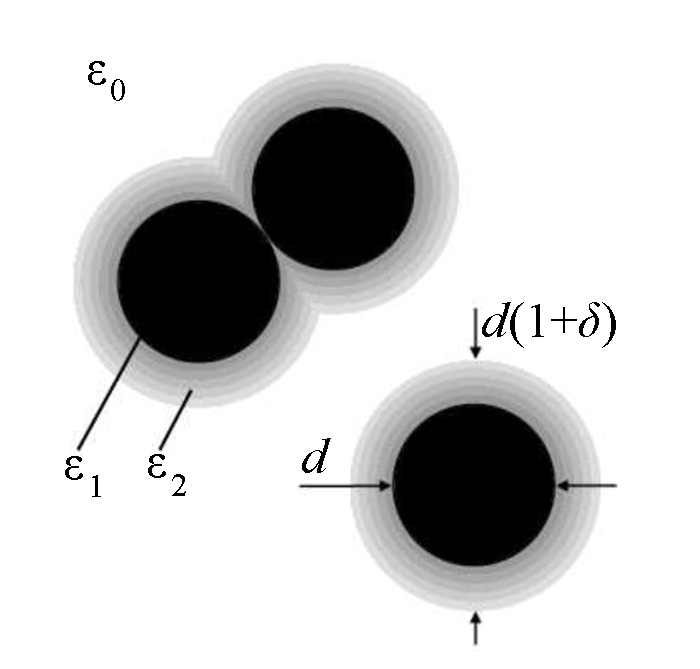
\includegraphics[width=0.35\textwidth]{images/particles-pen.eps}\\
    \includegraphics[width=0.35\textwidth]{images/2shell.png}
    % \includegraphics[width=0.35\textwidth]{images/CGA0-right.eps}
    % \begin{overpic}[width=0.3\textwidth]{images/CGA2-rot-1.eps}
    %              \put(15,85){$\cal{D}$}
    %              \put(20,35){$\cal{M}$}
    %              \put(35,30){$\cal{D}$}
    %              \put(48.5,42){$\cal{S}$}
    %              \put(75,0.7){$d$}
    %              \put(25,90){$d(1+\delta)$}
    %              \put(75,0.7){$\hat{\varepsilon}_0$}
    %              \put(75,0.7){$\hat{\varepsilon}_1$}
    %              \put(75,0.7){$\hat{\varepsilon}_2$}
    % \end{overpic}
  \end{center}
\vspace{-55pt}
\end{wrapfigure}

% \begin{figure}
%   \begin{center}
%             \begin{overpic}[width=0.7\textwidth]{images/CGA2.eps}
%                  \put(10,35){$\cal{D}$}
%                  \put(57,40){$\cal{M}$}
%                  \put(70,35){$\cal{D}$}
%                  \put(48.5,25){$\cal{S}$}
%                  \put(75,0.7){$L \ll \lambda$}
%             \end{overpic}
%     %\vspace{-10pt}
%   \end{center}
% \end{figure}

\footnotesize
Розглядаємо \textbf{макроскопічно однорідні та ізотропні дисперсні системи частинок із морфологією тверде ядро--проникна оболонка.}

\vspace{-5pt}
Локальне значення діелектричної проникності:
\vspace{-15pt}

$$
    \hat{\varepsilon}({\bf r}) = \left\{ 
    \begin{array}{ll}
    \hat{\varepsilon}_1, l<R_1 & l = \min\limits_{1 \leq a \leq N} |{\bf r} - {\bf r}_a| \\
    \hat{\varepsilon}_2, R_1 < l < R_2 & R_1 = d/2 \\
    \hat{\varepsilon}_0, l > R_2 & R_2 = d(1+\delta)/2
    \end{array}    
    \right. 
$$

Узагальнення на випадок неоднорідних оболонок з домінуванням ближчих шарів над дальніми.
\begin{equation*}\label{eq:distr1}
\hat{\varepsilon}({\bf r})=\begin{cases}
\hat{\varepsilon}_1, & l<R_1, \qquad l=\min\limits_{1 \leq a \leq N} |{\bf r} - {\bf r}_a| \\
\hat{\varepsilon}_{2,1}, &  R_1<l<R_{2,1},\\
{\hat{\varepsilon}_{2,m}}, & { R_{2,m-1}<l<R_{2,m}, \,2 \leq m \leq M},\\
\hat{\varepsilon}_0, & l>R_{2,M}.
\end{cases}
\end{equation*}

Частота тестуючого поля $\omega$ достатньо мала, щоб можна було знехтувати діелектричними втратами, тоді структура комплексної діелектричної проникності має вигляд: 
\vspace{-5pt}
$$
    \hat{\varepsilon} = \varepsilon + i \frac{4\pi\sigma}{\omega},
$$
де $\varepsilon$ -- дійсна частина діелектричної проникності; $\sigma$ -- статична провідність.

\end{frame}


%%%%%%%%%%%%%%%%%%%%%%%%%%%%%%%%%%%%%%%%%%%%%%%%%%%%%%%%%%%%%%%%%%%%%%%%%%%%%%%%%
\section{Процедура знаходження ефективних електричних параметрів}%%%%%%%%%%%%%%%%%%%%%%
%%%%%%%%%%%%%%%%%%%%%%%%%%%%%%%%%%%%%%%%%%%%%%%%%%%%%%%%%%%%%%%%%%%%%%%%%%%
\begin{frame}{Основні припущення та співвідношення}

\scriptsize
%\vspace{-10pt}
\begin{figure}
          \begin{center}
            \begin{overpic}[width=0.7\textwidth]{images/CGA.eps}
                 \put(2,40){$\cal{D}$}
                 \put(57,40){$\cal{M}$}
                 \put(70,35){$\cal{D}$}
                 \put(48.5,25){$\cal{S}$}
                 \put(75,0.7){$L \ll \lambda$}
            \end{overpic}
          \end{center}
\end{figure}

\begin{list}{$\bullet$}{\leftmargin=1em \itemindent=0em}\footnotesize

\item 
Електричний відгук дисперсної системи $\cal{D}$ еквівалентний відгуку допоміжної системи $\cal{S}$, утвореної диспергуванням компонентів $\cal{D}$ в деяку однорідну матрицю $\cal{M}$ з проникністю $\hat{\varepsilon}_{\rm f}$.

\item
$\cal{S}$ -- сукупуність макроскопічних областей (компактних груп) з лінійними розмірами $L \ll \lambda$ в $\cal{M}$, які є фактично точками по відношенню до $\lambda$.

\item
Розподіл комплексної діелектричної проникності в $\cal{S}$:
$$
    \hat{\varepsilon} ({\bf r}) = \hat{\varepsilon}_{\rm f} + \delta\hat{\varepsilon} ({\bf r}),
$$
де $\delta\hat{\varepsilon} ({\bf r})$ -- внесок компактної групи, розташованої в точці $\bf r$.

\item 
Ефективна $\hat{\varepsilon}_{\rm eff}$ визначається із співвідношення
\begin{equation}\label{eq:effcomplex} 
\langle {\bf{J}} ({\bf{r}})\rangle =
-i\frac{\omega}{4\pi}\langle \hat{\varepsilon} ({\bf{r}}) {\bf{E}}
({\bf{r}}) \rangle = -i\frac{\omega}{4\pi} \hat{\varepsilon}_{\rm
eff} \langle {\bf{E}} ({\bf{r}}) \rangle,
\end{equation}
${\bf J}({\bf{r}})$ та ${\bf E}({\bf{r}})$ -- локальні значення густини комплексних струму та поля.

\end{list}

\end{frame}

%%%%%%%%%%%%%%%%%%%%%%%%%%%%%%%%%%%%%%%%%%%%%%%%%%%%%
\begin{frame}{Алгоритм обчислення ${\bf E} ({\bf r})$}
\footnotesize
%[М.Я. Сушко, ЖЭТФ {\bf 132} (2007) 478; J. Phys. D: Appl. Phys. {\bf 42} (2009) 155410; Phys. Rev. E {\bf 96} (2017) 062121]

\begin{list}{$\bullet$}{\leftmargin=1em \itemindent=0em}

% \item 
% Ефективна $\hat{\varepsilon}_{\rm eff}$ визначається із співвідношення
% \begin{equation}\label{eq:effcomplex} 
% \langle {\bf{J}} ({\bf{r}})\rangle =
% -i\frac{\omega}{4\pi}\langle \hat{\varepsilon} ({\bf{r}}) {\bf{E}}
% ({\bf{r}}) \rangle = -i\frac{\omega}{4\pi} \hat{\varepsilon}_{\rm
% eff} \langle {\bf{E}} ({\bf{r}}) \rangle,
% \end{equation}
% ${\bf J}({\bf{r}})$ та ${\bf E}({\bf{r}})$ -- локальні значення густини комплексних струму та поля.


\item 
Рівняння поширення електромагнітного поля в неоднорідному середовищі:
\begin{equation} \label{eq:propogating_field}
\Delta {\bf E} + k_0^{2}\hat{\varepsilon}_{\rm f} {\bf E} - {\rm
grad}\, {\rm div} {\bf E} = - k_{0}^{2} \delta
\hat{\varepsilon} {\bf E},
\end{equation}
де $k_0=\omega/c$ -- модуль хвильового вектора ${\bf k}_0$ у вакуумі.


\item
Еквівалентне інтегральне рівняння
\begin{equation}\label{eq:propogating_field_integral} 
{\rm {\bf E}}({\rm {\bf r}}) = {\rm {\bf E}}_{0} ({\rm
{\bf r}}) - {\int\limits_{V} {d{\rm {\bf {r}'}}\,}} {\rm T}(|{\rm {\bf
r}}-{\rm {\bf {r}'}}|) k_{0}^{2} \delta \hat{\varepsilon} ({\rm
{\bf {r}'}})\,{\rm {\bf E}}({\rm {\bf {r}'}}),
\end{equation}
де ${\bf E}_0 ({\bf r}) = {\bf E}_0 \exp{(i\, {\bf k} \cdot{\bf r})}$ та ${\bf k} = \hat{\varepsilon}_{\rm f}^{1/2} {\bf k}_0$ (з ${\rm Im}{\hat{\varepsilon}_{\rm f}}^{1/2} \geq 0$) -- поле та хвильовий вектор падаючої хвилі в $\cal{M}$;
${\rm T}(r)$ -- пропагатор електричного поля. 

\item
Підінтегральний пропагатор ${\rm T}(r)$ заміняється розкладом на сингулярну та головну частини [W. Weiglhofer, Am. J. Phys. {\bf 57} (1989) 455]:
\begin{eqnarray}\label{eq:propog_representation} 
&&{\widetilde T}_{\alpha\beta} ({\rm {\bf
r}}) = \frac{1}{3k^{2}} \delta_{\alpha\beta} \delta ({\rm {\bf
r}})\,e^{ikr} + \frac{1}{4\pi k^{2}}
\left(\frac{1}{r^3}-\frac{ik}{r^2}\right)\nonumber\\
&&\times\left( \delta _{\alpha\beta} - 3e_{\alpha} e_{\beta}
\right)\,e^{ikr} - \frac{1}{4\pi r}\left( {\delta _{\alpha\beta} -
e_{\alpha} e_{\beta}} \right)\,e^{ikr},\quad 
e_\alpha = r_\alpha/|{\bf r}|.
\end{eqnarray}

\end{list}

\end{frame}


%%%%%%%%%%%%%%%%%%%%%%%%%%%%%%%%%%%%%%%%%%%
\begin{frame}{Знаходження $\hat{\varepsilon}_{\rm f}$ та загальне співвідношення для $\hat{\varepsilon}_{\rm eff}$}
\footnotesize

\begin{list}{$\bullet$}{\leftmargin=1em \itemindent=0em}

\item
Після переходу до квазістатичного наближення із урахуванням симетрії парних кореляційних функцій для розглядуваних систем отримуємо:
\begin{equation}\label{eq:Eaveraged}
\langle \mathbf{E} (\mathbf{r}) \rangle = \left\langle \frac{ 3
\hat{\varepsilon}_{\rm f}  }{3 \hat{\varepsilon}_{\rm f}
+ \delta\hat{\varepsilon}({\bf r})} \right\rangle \mathbf{E}_0 ,
\end{equation}
\begin{equation}\label{eq:Caveraged}
\langle \mathbf{J}  (\mathbf{r}) \rangle = -i \frac{\omega}{4\pi}
\, \hat{\varepsilon}_{\rm f}\left[1+ 2\left\langle \frac{
\delta\hat{\varepsilon}({\bf r}) }{3 \hat{\varepsilon}_{\rm f}
+ \delta\hat{\varepsilon}({\bf r})} \right\rangle \right] \mathbf{E}_0.
\end{equation}

\item
З граничних умов для нормальних компонент електричного поля на поверхні розділу $\cal{M}$ та $\cal{D}$:
\begin{equation} \label{eq:boundarycondition}
\hat{\varepsilon}_{\rm
f} {\mathbf{E}}_{0n} = \hat{\varepsilon}_{\rm eff}
\left\langle{\mathbf{E}}({\mathbf{r}})\right\rangle_n.
\end{equation}
За умови, що $\hat{\varepsilon}_{\rm f} \neq 0$, дістаємо:
\begin{equation} \label{eq:ef} 
\hat{ \varepsilon}_{\rm f} = \hat{ \varepsilon}_{\rm eff},
\end{equation}
що дає рівняння для знаходження $\hat{\varepsilon}_{\rm eff}$:
\begin{equation} \label{eq:equation}
\boxed{
\left\langle \frac{\delta\hat{\varepsilon}({\bf r}) }{3 \hat{\varepsilon}_{\rm eff} + \delta\hat{\varepsilon}({\bf r})} \right\rangle = 0.
}
\end{equation}

До цього місця структура частинок не використовується взагалі.

\end{list}

\end{frame}

%%%%%%%%%%%%%%%%%%%%%%%%%%%%%%%%%%%%%%%%%%%%%%%%%%%%%
\begin{frame}{Моделювання $\delta\hat{\varepsilon}({\bf r})$}
\footnotesize

\begin{wrapfigure}{r}{0.4\textwidth}
\vspace{-20pt}
  \begin{center}
    \includegraphics[width=0.4\textwidth]{images/Fig1_Microstructure_new5.eps}
  \end{center}
\vspace{-30pt}
\end{wrapfigure}

Для випадку $\hat{\varepsilon}_2 = const$:
\begin{equation*}
\begin{split}
    \delta\hat{\varepsilon}({\bf r}) = [1 - \Pi_2({\bf r})]\Delta\hat{\varepsilon}_0 + \Pi_1({\bf r}) \Delta\hat{\varepsilon}_1\\ 
    + [\Pi_2({\bf r}) - \Pi_1({\bf r})]\Delta\hat{\varepsilon}_2,
\end{split}
\end{equation*}
де $\Delta\hat{\varepsilon}_q = \hat{\varepsilon}_{q} - \hat{\varepsilon}_{\rm f}\, (q=0,1,2),$ та введено такі характеристичні функції: \\
$\cdot\quad \Pi_1 ({\bf r}) = \sum\limits_{a=1}^N \chi_a^{(1)} ({\bf r})$~--~області, зайняті твердими ядрами ($\chi_a^{(1)}({\bf r})$ -- характеристична функція ядра $a$-ої частинки);\\
$\cdot\quad \Pi_2 ({\bf r}) = 1 - \prod\limits_{a=1}^N [1 - \chi_a^{(2)} ({\bf r})]$~--~області, зайнятої твердими ядрами разом з проникними оболонками ($\chi_a^{(2)}({\bf r})$ -- характеристична функція $a$-ої частинки (її ядра та оболонки)).

Для неоднорідних оболонок:
\begin{equation*}
\begin{split}
\delta\hat{\varepsilon} ({\bf r}) = \left[1- \Pi_{2,M}({\bf
r})\right] \Delta\hat{\varepsilon}_0
+ \Pi_1({\bf r}) \Delta\hat{\varepsilon}_1
+  \left[\Pi_{2,1}({\bf r})
-\Pi_1({\bf r})  \right] \Delta\hat{\varepsilon}_{2,1} \\
+ {\sum\limits_{m=2}^M  \left[ \Pi_{2,m}({\bf r}) -
\Pi_{2,m-1}({\bf r}) \right] \Delta\hat{\varepsilon}_{2,m}}.
\end{split}
\end{equation*}
% де $\Pi_{2,m} ({\bf r}) = 1 - \prod\limits_{a=1}^N [1 - \chi_a^{(2,m)} ({\bf r})]$ -- характеристична функція області, зайнятої твердими ядрами разом з $m$-ими проникними оболонками ($\chi_a^{(2,m)}({\bf r})$ -- характеристична функція $a$-ого ядра та його $m$-ої оболонки).

\end{frame}

%%%%%%%%%%%%%%%%%%%%%%%%%%%%%%%%%%%%%%%%%%%%%%%%%%%%%
\begin{frame}{Основні результати}
\footnotesize

\begin{list}{$\bullet$}{\leftmargin=1em \itemindent=0em}
\item
Рівняння для $\hat{\varepsilon}_{\rm eff}$ у випадку \textbf{однорідних оболонок}:
\begin{equation}\label{eq:uniformshell}
\boxed{
\left[1-\phi(c, \delta)\right]\frac{\hat{\varepsilon}_0
-\hat{\varepsilon}_{\rm eff}}{2\hat{\varepsilon}_{\rm
eff}+\hat{\varepsilon}_0} + c\,\frac{\hat{\varepsilon}_1
-\hat{\varepsilon}_{\rm eff}}{2\hat{\varepsilon}_{\rm
eff}+\hat{\varepsilon}_1}
+\left[\phi(c, \delta)-c\right]\frac{\hat{\varepsilon}_2
-\hat{\varepsilon}_{\rm eff}}{2\hat{\varepsilon}_{\rm
eff}+\hat{\varepsilon}_2}=0, 
}
\end{equation}
де $c = \langle \Pi_1 \rangle$ -- об'ємна концентрація ядер; $\phi = \langle \Pi_2 \rangle$ -- об'ємна концентрація ядер з оболонками. 

\item
Для \textbf{неоднорідних оболонок} після переходу до границі $M \to \infty$ ($\delta_M = const$):
\begin{equation}\label{eq:nonuniformshell}
\boxed{
\left[1-\phi(c, \delta_M)\right]\frac{\hat{\varepsilon}_0
-\hat{\varepsilon}_{\rm eff}}{2\hat{\varepsilon} _{\rm
eff}+\hat{\varepsilon}_0}+ c\,\frac{\hat{\varepsilon}_1
-\hat{\varepsilon}_{\rm eff}}{2\hat{\varepsilon}_{\rm
eff}+\hat{\varepsilon}_1}
+\int\limits_0^{\delta_M}\frac{\partial \phi(c,u)}{\partial
u}\frac{\hat{\varepsilon}_2 (u) -\hat{\varepsilon}_{\rm
eff}}{2\hat{\varepsilon}_{\rm eff}+\hat{\varepsilon}_2 (u)}\,du
=0
}
\end{equation}

\item
За умови, що  $|\sigma_{\rm eff}-\sigma_{ q}|  \gg  
\left(2\varepsilon_{\rm eff} +\varepsilon_q \right) \omega/4\pi$ для всіх $q=0,1,2$,  рівняння для квазістатичної провідності мають вигляд:
\begin{equation*}\label{eq:conductivity}
\boxed{
\left[1-\phi(c, \delta)\right]\frac{\sigma_0 -\sigma_{\rm
eff}}{2\sigma_{\rm eff}+\sigma_0} + c\,\frac{\sigma_1 -\sigma_{\rm
eff}}{2\sigma_{\rm eff}+\sigma_1} 
+\left[\phi(c, \delta)-c\right]\frac{\sigma_2 -\sigma_{\rm
eff}}{2\sigma_{\rm eff}+\sigma_2}=0. 
}
\end{equation*}
\begin{equation*}\label{eq:nonuniformconductivity}
\boxed{
\left[1-\phi(c, \delta_M)\right]\frac{\sigma_0 -\sigma_{\rm
eff}}{2\sigma _{\rm eff}+\sigma_0}+ c\,\frac{\sigma_1 -\sigma_{\rm
eff}}{2\sigma_{\rm eff}+\sigma_1} 
+\int\limits_0^{\delta_M}\frac{\partial \phi(c,u)}{\partial
u}\frac{\sigma_2 (u) -\sigma_{\rm eff}}{2\sigma_{\rm eff}+\sigma_2
(u)}\,du =0.
}
\end{equation*}
У статичному випадку цей результат є \textbf{строгим}.

\end{list}

\end{frame}


%%%%%%%%%%%%%%%%%%%%%%%%%%%%%%%%%%%%%%%%%%%%%%%%%%%%%%%%%%%%%%%%%%%%%%%%%%%%%%%%%%%%%%%%%%%
\section{Тестування моделі на результатах числових симуляцій}%%%%%%%%%%%%%%%%%%%%%%%%%%%%%%%
%%%%%%%%%%%%%%%%%%%%%%%%%%%%%%%%%%%%%%%%%%%%%%%%%%%%%%%%%%%%%%%%%%%%%%%%%%%%%%%%%%%%%%%%%%

\begin{frame}{Тестування теорії на результатах симуляцій RRN}

{\footnotesize
Симуляції: [M. Siekierski et al., Electrochimica Acta {\bf 50} (2005) 3796; 
J. New Mat. Electrochem. Systems {\bf 9} (2006) 375;
J. Pow. Sour. {\bf 173} (2007) 748]
}

\begin{figure}[tb]
    \centering
    \includegraphics[width=0.7\textwidth]{images/RRN.png}
    \caption{Схематичне зображення алгоритму Random Resistor Network (RRN): a) модельна система типу ядро-оболонка; b) її апроксимація системою кубів; c) отримана тривимірна кубічна гратка резисторів.\\ {\footnotesize (Рис. взято з [M. Siekierski, K. Nadara, J. Pow. Sour. {\bf 173} (2007) 748])}}
\end{figure}
\vspace{-10pt}
Концентрації ядер в системах a) та b) рівні: $c=c'$, тоді відповідні відносні товщини будуть зв'язані співвідношенням:
$$
    \delta = K\delta'
$$
$$
    k \leq K \leq 1, \qquad k=(\pi/6)^{1/3}
$$

\end{frame}

%%%%%%%%%%%%%%%%%%%%%%%%%%%%%%%%%%%%%%%%%%%%%%%%%%%%%
%{\setbeamertemplate{frame footer}{Симуляції: [M. Siekierski, K. Nadara, J. Pow. Sour. {\bf 173} (2007) 748]}
\begin{frame}{Тестування зв'язку геометричних параметрів моделей a) та b)}

{ Об'ємні концентрації оболонок товщиною $t=5$~мкм як функції $c$.}
\vspace{-5pt}

\scriptsize{Симуляції: [M. Siekierski, K. Nadara, J. Pow. Sour. {\bf 173} (2007) 748]}
\vspace{-5pt}

\footnotesize
\begin{columns}[T,onlytextwidth]
    \column{0.5\textwidth}
      \begin{figure}
        \centering
        \qquad Діаметр ядра $d=7$~мкм
        \includegraphics[width=0.99\textwidth]{images/Fig2_SiekierskiShell_107.eps}
      \end{figure}

    \column{0.5\textwidth}
      \begin{figure}
        \centering
        \qquad Діаметри ядер $d=3,5,9$~мкм
        \includegraphics[width=0.99\textwidth]{images/Fig3_SiekierskiShell_103-9.eps}
      \end{figure}
\end{columns}

\begin{columns}[T,onlytextwidth]
    \column{0.45\textwidth}
      \vspace{5pt}
    %   Середньоквадратична похибка:
    %   $$
    %     \Delta_a = \sqrt{\frac{1}{N}\sum\limits_{i=1}^N (a_i - \tilde{a}_i)^2}
    %   $$
    Для сферичних частинок $\phi$ знайдено статистичними методами в рамках суперпозиційного підходу Кірквуда, строгого на рівні третього вірального коефіцієнта  [P.~Rikvold, G.~Stell, J. Coll. and Int. Sci. {\bf 108} (1985) 158]

    \column{0.55\textwidth}
    %   \begin{table}
    %     %\caption{Largest cities in the world (source: Wikipedia)}
    %     \begin{tabular}{ll}
    %       \toprule
    %       Експеримент & MSE\\
    %       \midrule
    %       $\circ$ $t=0$~мкм & 0.0024\\
    %       $\blacklozenge$ $d=3$~мкм & 0.0053\\
    %       $\blacksquare$ $d=5$~мкм & 0.011\\
    %       $\blacktriangle$ $d=7$~мкм & 0.014\\
    %       $\bullet$ $d=9$~мкм & 0.0097\\
    %       \bottomrule
    %     \end{tabular}
    %   \end{table}
    \begin{equation*}\label{effectiveconcentration}
    \begin{split}
    \phi(c,\delta)= 1-
    (1 - c)\,\exp\left[{-\frac{((1+\delta)^3 -
    1)c}{1-c}}\right] \\
     \times  \exp\left\{
    - \frac{3(1 + \delta)^3
    c^2}{2(1 - c)^3} \left[2 - \frac{3}{1+\delta} +
    \frac{1}{(1+\delta)^3} \right. \right. \\
    - \left. \left. \left( \frac{3}{1+\delta} -
    \frac{6}{(1+\delta)^2} + \frac{3}{(1+\delta)^3}\right) c
    \right]\right\}. 
    \end{split}
    \end{equation*}
\end{columns}

\end{frame}
%}
%%%%%%%%%%%%%%%%%%%%%%%%%%%%%%%%%%%%%%%%%%%%%%%%%%%%%
%{\setbeamertemplate{frame footer}{Симуляції: [M. Siekierski, K. Nadara, Electrochimica Acta {\bf 50} (2005) 3796]}
\begin{frame}{Порівняння з числовими даними з провідності}
Концентраційна залежність ефективної провідності при фіксованих $t$ (зліва) та $d$ (справа) з різними значеннями $K$.
\vspace{-5pt}

\scriptsize{Симуляції: [M. Siekierski, K. Nadara, Electrochimica Acta {\bf 50} (2005) 3796]}

\footnotesize
\begin{columns}[T,onlytextwidth]
    \column{0.5\textwidth}
      \begin{figure}
        \centering
        { \qquad Товщина оболонки $t=5$~мкм}
        \includegraphics[width=0.99\textwidth]{images/Fig6_Siekierski_HomogeneousLayers_t_fixed.eps}
      \end{figure}

    \column{0.5\textwidth}
      \begin{figure}
        \centering
        { \qquad Діаметр ядра $d=5$~мкм}
        \includegraphics[width=0.99\textwidth]{images/Fig7_Siekierski_HomogeneousLayers_d_fixed.eps}
      \end{figure}
\end{columns}

\begin{columns}[T,onlytextwidth]
    \column{0.6\textwidth}
      \vspace{10pt}
      Середньоквадратична відносна похибка:
      $$
        \bar{\Delta}_a = \sqrt{\frac{1}{N}\sum\limits_{i=1}^N \left( \frac{a_i - \tilde{a}_i}{a_i} \right)^2}
      $$

    \column{0.4\textwidth}
      \begin{table}
        %\caption{Largest cities in the world (source: Wikipedia)}
        \begin{tabular}{ll}
          \toprule
          Експеримент & $\max \bar{\Delta}_{\sigma_{\rm eff}/\sigma_0}$\\
          \midrule
          $t=5$~мкм & 0.40 | 0.048\\
          $d=5$~мкм & 0.35 | 0.019\\
          \bottomrule
        \end{tabular}
      \end{table}
\end{columns}
\end{frame}
%}

%%%%%%%%%%%%%%%%%%%%%%%%%%%%%%%%%%%%%%%%%%%%%%%%%%%%%
%{\setbeamertemplate{frame footer}{Симуляції: [M. Siekierski et al., J. New Mat. Electrochem. Systems {\bf 9} (2006) 375]}
\begin{frame}{Тестування моделі для випадку неоднорідних оболонок}
Концентраційна залежність ефективної провідності з різними значеннями $K$ для гаусового профілю оболонок.
\vspace{-5pt}

\scriptsize{Симуляції: [M. Siekierski et al., J. New Mat. Electrochem. Systems {\bf 9} (2006) 375]}

\footnotesize
\begin{columns}[T,onlytextwidth]
    \column{0.5\textwidth}
      \begin{figure}
        \centering
        { \qquad Товщина оболонки $t=5$~мкм}
        \includegraphics[width=0.99\textwidth]{images/Fig10_Siekierski_t_fixed.eps}
        $\max \bar{\Delta}_{\sigma_{\rm eff}/\sigma_0} \approx 0.41\,|\,0.048$\\
      \end{figure}

    \column{0.5\textwidth}
      \begin{figure}
        \centering
        { \qquad Діаметр ядра $d=5$~мкм}
        \includegraphics[width=0.99\textwidth]{images/Fig11_Siekierski_d_fixed.eps}
        $\max \bar{\Delta}_{\sigma_{\rm eff}/\sigma_0} \approx 0.28\,|\,0.28$
      \end{figure}
\end{columns}

\end{frame}
%}

%%%%%%%%%%%%%%%%%%%%%%%%%%%%%%%%%%%%%%%%%%%%%%%%%%%%%%%%%%%%%%%%%%%%%%%%%%%%%%%%%%%%%%%%%%%
\section{Застосування моделі до аналізу ефективної провідності композитних електролітів}%%%%%%%%%%%%%%%%%%%%%%%%%%%%%%%
%%%%%%%%%%%%%%%%%%%%%%%%%%%%%%%%%%%%%%%%%%%%%%%%%%%%%%%%%%%%%%%%%%%%%%%%%%%%%%%%%%%%%%%%%%
%\subsection{Тестування моделі на числових результатах симуляцій}

%%%%%%%%%%%%%%%%%%%%%%%%%%%%%%%%%%%%%%%%%%%%%%%%%%%%%
%\subsection{Порівняння з експериментальними даними}

%{\setbeamertemplate{frame footer}{Експеримент: [C.C. Liang, J. Electrochem. Soc., {\bf 120} (1973) 1289]}
\begin{frame}{Порівняння теорії з експериментальними даними -- 1}
Концентраційна залежність провідності систем $\rm LiI-Al_2O_3$.
\vspace{-5pt}

\scriptsize{Експеримент: [C.C. Liang, J. Electrochem. Soc., {\bf 120} (1973) 1289]}
\vspace{-10pt}

\footnotesize
\begin{columns}[T,onlytextwidth]
    \column{0.5\textwidth}
      \begin{figure}
        \centering
        %{ \qquad Діаметр ядра $d=7$~мкм}
        %\includegraphics[width=0.99\textwidth]{images/Fig12_Liang_LiI-Al2O3-Processing.eps}
        \begin{overpic}[width=0.95\textwidth]{images/Fig12_Liang_LiI-Al2O3-Processing.eps}
                 \put(45,87){\scriptsize $\sigma_0 \approx 2.5 \times 10^{-7}$~С/см}
        \end{overpic}
      \end{figure}
      \vspace{-10pt}
      % подвійні оболонки - $\bar{\Delta}_{\sigma_{\rm eff}/\sigma_0} \approx 0.143$\\
      % неперервний профіль - $\bar{\Delta}_{\sigma_{\rm eff}/\sigma_0} \approx 0.163$
      Точкова лінія -- електрично однорідна оболонка.\\
      Штрихована лінія -- подвійна (ступінчата) оболонка.\\
      Неперервна лінія -- гладкий профіль провідності.
      

    \column{0.5\textwidth}
    \vspace{5pt}
        \begin{tikzpicture}
            \node[anchor=south west,inner sep=0] (image) at (0,0) {\includegraphics[width=0.95\textwidth]{images/Fig13_Liang_LiI-Al2O3-Profile.eps}};
            \begin{scope}[x={(image.south east)},y={(image.north west)}]
                \node[] at (0.55,1.05) {Одночастинковий профіль провідності};
            \end{scope}
        \end{tikzpicture}
        Концентраційна залежність провідності матриці $\sigma_0^*$:
        \vspace{-5pt}
        \begin{eqnarray*}
        &&(1 - \phi(c,\delta_1))\frac{\sigma_0^* - \sigma_{\rm
        eff}}{2\sigma_{\rm eff} + \sigma_0^*}=\nonumber\\
        &&(1 - \phi(c,\delta_2))
        \frac{\sigma_0 - \sigma_{\rm eff}}{2\sigma_{\rm eff} + \sigma_0}
         \nonumber\\
        &&+ (\phi(c,\delta_2) - \phi(c,\delta_1)) \frac{\sigma_{2,2} -
        \sigma_{\rm eff}}{2\sigma_{\rm eff} + \sigma_{2,2}}
        \end{eqnarray*}
      
\end{columns}

\end{frame}
%}
\begin{frame}{Порівняння теорії з експериментальними даними -- 1}
Концентраційна залежність провідності систем $\rm LiI-Al_2O_3$.
\vspace{-5pt}

\scriptsize{Експеримент: [C.C. Liang, J. Electrochem. Soc., {\bf 120} (1973) 1289]}
\vspace{-10pt}

\footnotesize
\begin{columns}[T,onlytextwidth]
    \column{0.5\textwidth}
      \begin{figure}
        \centering
        %{ \qquad Діаметр ядра $d=7$~мкм}
        %\includegraphics[width=0.99\textwidth]{images/Fig12_Liang_LiI-Al2O3-Processing.eps}
        \begin{overpic}[width=0.95\textwidth]{images/Fig12_Liang_LiI-Al2O3-Processing.eps}
                 \put(45,87){\scriptsize $\sigma_0 \approx 2.5 \times 10^{-7}$~С/см}
        \end{overpic}
      \end{figure}
      \vspace{-10pt}
      % подвійні оболонки - $\bar{\Delta}_{\sigma_{\rm eff}/\sigma_0} \approx 0.143$\\
      % неперервний профіль - $\bar{\Delta}_{\sigma_{\rm eff}/\sigma_0} \approx 0.163$
      Точкова лінія -- електрично однорідна оболонка.\\
      Штрихована лінія -- подвійна (ступінчата) оболонка.\\
      Неперервна лінія -- гладкий профіль провідності.
      

    \column{0.5\textwidth}
    \vspace{5pt}
        \begin{tikzpicture}
            \node[anchor=south west,inner sep=0] (image) at (0,0) {\includegraphics[width=0.95\textwidth]{images/Fig13_Liang_LiI-Al2O3-Profile.eps}};
            \begin{scope}[x={(image.south east)},y={(image.north west)}]
                %\draw[red,ultra thick,rounded corners] (0.62,0.65) rectangle (0.78,0.75);
                \node[] at (0.55,1.05) {Одночастинковий профіль провідності};
                \draw[red, thick] (0.6,0.2) ellipse (0.25 and 0.05);
                \draw[red, thick] (0.3,0.58) ellipse (0.1 and 0.4);
                \draw[->, thick, red] (0.55,0.7) -- (0.4,0.55);
                \draw[->, thick, red] (0.65,0.4) -- (0.6,0.25);
                \node[red] at (0.7,0.72) {Оболонка};
                \node[red] at (0.67,0.45) {Матриця};
            \end{scope}
        \end{tikzpicture}
        \vspace{-20pt}
      \begin{figure}
        \centering
        %{Одночастинковий профіль провідності}
        %\includegraphics[width=0.95\textwidth]{images/Fig13_Liang_LiI-Al2O3-Profile.eps}\\
        \includegraphics[width=0.75\textwidth]{images/Fig14_Liang_LiI-Al2O3-Matrix_2.eps}
      \end{figure}
      
\end{columns}

\end{frame}
%%%%%%%%%%%%%%%%%%%%%%%%%%%%%%%%%%%%%%%%%%%%%%%%%%%%%
%{\setbeamertemplate{frame footer}{Експеримент: [W. Wieczorek, M. Siekierski, J. Appl. Phys. {\bf 76} (1994) 2220;\par J. Przyluski, M. Siekierski, W. Wieczorek, Electrichimica A. {\bf 40} (1995) 2101]}
\begin{frame}{Порівняння теорії з експериментальними даними -- 2}
Ефективна провідність полімерних композитних електролітів $\rm (PEO)NaI-NASICON$ та $\rm (PEO)NaI-\theta Al_2O_3$.
\vspace{-5pt}

\scriptsize{Експеримент: [W. Wieczorek, M. Siekierski, J. Appl. Phys. {\bf 76} (1994) 2220; J. Przyluski, M. Siekierski, W. Wieczorek, Electrichimica A. {\bf 40} (1995) 2101]}
\vspace{-5pt}

\footnotesize
\begin{columns}[T,onlytextwidth]
    \column{0.5\textwidth}
      \begin{figure}
        \centering
        %{ \qquad Діаметр ядра $d=7$~мкм}
        \includegraphics[width=0.99\textwidth]{images/Fig2_PEO-NaI_NASICON_PEO-NaI-theta-Al2O3.eps}
        % 1d -- $\bar{\Delta}_{\sigma_{\rm eff}/\sigma_0} \approx 0.17$\\
        % 2d -- $\bar{\Delta}_{\sigma_{\rm eff}/\sigma_0} \approx 0.37$
      \end{figure}

    \column{0.5\textwidth}
      \begin{figure}
        %\centering
        \vspace{-10pt}
        { \qquad Одночастинкові профілі провідності}
          \begin{center}
            \begin{overpic}[width=0.99\textwidth]{images/Fig2_PEO-NaI_NASICON_Profile.eps}
                 \put(45,50){\scriptsize $\sigma_0 = 9.86 \times 10^{-9}$~С/см}
            \end{overpic}
            \begin{overpic}[width=0.99\textwidth]{images/Fig2_PEO-NaI-theta-Al2O3_Profile.eps}
                 \put(45,15){\scriptsize $\sigma_0 = 1.54 \times 10^{-8}$~С/см}
            \end{overpic}
          \end{center}
        %\includegraphics[width=0.99\textwidth]{images/Fig2_PEO-NaI_NASICON_Profile.eps}
        %\includegraphics[width=0.99\textwidth]{images/Fig2_PEO-NaI-theta-Al2O3_Profile.eps}
      \end{figure}
      
\end{columns}

\end{frame}
%}
%%%%%%%%%%%%%%%%%%%%%%%%%%%%%%%%%%%%%%%%%%%%%%%%%%%%%
%{\setbeamertemplate{frame footer}{Експеримент: [W. Wieczorek, M. Siekierski, J. Appl. Phys. {\bf 76} (1994) 2220;\par W. Wieczorek et al, J. Phys. Chem. {\bf 98} (1994) 6840]}
\begin{frame}{Порівняння теорії з експериментальними даними -- 3}
Ефективна провідність полімерних композитних електролітів $\rm (PEO)LiClO_4-PAAM$ та $\rm (OMPEO)LiClO_4-PAAM$.
\vspace{-5pt}

\scriptsize{Експеримент: [W. Wieczorek, M. Siekierski, J. Appl. Phys. {\bf 76} (1994) 2220; W. Wieczorek et al, J. Phys. Chem. {\bf 98} (1994) 6840]}
\vspace{-5pt}

\footnotesize
\begin{columns}[T,onlytextwidth]
    \column{0.5\textwidth}
      \begin{figure}
        \centering
        %{ \qquad Діаметр ядра $d=7$~мкм}
        \includegraphics[width=0.99\textwidth]{images/Fig3_PEO-PAAM_LiClO4_OMPEO-PAAM_LiClO4.eps}
        % 3c -- $\bar{\Delta}_{\sigma_{\rm eff}/\sigma_0} \approx 0.29$\\
        % 4c -- $\bar{\Delta}_{\sigma_{\rm eff}/\sigma_0} \approx 0.33$
      \end{figure}

    \column{0.5\textwidth}
      \begin{figure}
        %\centering
        \vspace{-10pt}
        { \qquad Одночастинкові профілі провідності}
        %\includegraphics[width=0.99\textwidth]{images/Fig3_PEO-PAAM_LiClO4_Profile.eps}
        %$\sigma_0 = 13.1$~мкС/см
          \begin{center}
            \begin{overpic}[width=0.99\textwidth]{images/Fig3_PEO-PAAM_LiClO4_Profile.eps}
                 \put(45,15){\scriptsize $\sigma_0 = 6.21 \times 10^{-7}$~С/см}
            \end{overpic}
            \begin{overpic}[width=0.99\textwidth]{images/Fig3_OMPEO-PAAM_LiClO4_Profile.eps}
                 \put(45,15){\scriptsize $\sigma_0 = 1.61 \times 10^{-5}$~С/см}
            \end{overpic}
          \end{center}
        %\includegraphics[width=0.99\textwidth]{images/Fig3_OMPEO-PAAM_LiClO4_Profile.eps}
        %$\sigma_0 = 13.1$~мкС/см
      \end{figure}
      
\end{columns}

\end{frame}
%}
%%%%%%%%%%%%%%%%%%%%%%%%%%%%%%%%%%%%%%%%%%%%%%%%%%%%%
%{\setbeamertemplate{frame footer}{Експеримент: [W. Wieczorek, M. Siekierski, J. Appl. Phys. {\bf 76} (1994) 2220;\par W. Wieczorek et al, J. Phys. Chem. {\bf 98} (1994) 6840]}
\begin{frame}{Інтерпретація отриманого одночастинкового профілю}
Одночастиноквий профіль провідності отриманий для полімерних композитних електролітів $\rm (OMPEO)LiClO_4-PAAM$.

\footnotesize

\begin{tikzpicture}
            \node[anchor=south west,inner sep=0] (image) at (0,0) {\includegraphics[width=0.85\textwidth]{images/Fig3_OMPEO-PAAM_LiClO4_Profile.eps}};
            \begin{scope}[x={(image.south east)},y={(image.north west)}]
                \draw[red, very thick] (0.49,0.69) ellipse (0.08 and 0.05);
                \draw[red, very thick] (0.6,0.72) ellipse (0.07 and 0.3);
                \draw[red, very thick] (0.75,0.67) ellipse (0.12 and 0.06);
                \draw[->, thick, red] (0.35,0.8) -- (0.45,0.71);
                \node[red] at (0.3,0.95) {Stiffening effect;};
                \node[red] at (0.35,0.89) {нерегулярності форми;};
                \node[red] at (0.31,0.83) {непровідний шар};
                \draw[->, thick, red] (0.35,0.5) -- (0.6,0.6);
                \node[red] at (0.3,0.47) {Аморфізований};
                \node[red] at (0.25,0.41) {полімер};
                \draw[->, thick, red] (0.85,0.9) -- (0.75,0.67);
                \node[red] at (0.85,0.93) {Матричні ефекти};
            \end{scope}
\end{tikzpicture}

\end{frame}
%}
%%%%%%%%%%%%%%%%%%%%%%%%%%%%%%%%%%%%%%%%%%%%%%%%%%%%%
{\setbeamertemplate{frame footer}{Експеримент: [W. Wieczorek, M. Siekierski, J. Appl. Phys. {\bf 76} (1994) 2220;\par W. Wieczorek et al, J. Phys. Chem. {\bf 98} (1994) 6840]}
\begin{frame}{Порівняння з іншими теоріями}
Ефективна провідність полімерних композитних електролітів $\rm (PEO)LiClO_4-PAAM$ та $\rm (OMPEO)LiClO_4-PAAM$

\footnotesize
неперервні лінії -- наш підхід; 
штрихован лінії -- підхід Нана--Вєчорика


      \begin{figure}
        \centering
        %{ \qquad Діаметр ядра $d=7$~мкм}
        \includegraphics[width=0.6\textwidth]{images/Fig5_Comparison.eps}
      \end{figure}

\end{frame}
}
%%%%%%%%%%%%%%%%%%%%%%%%%%%%%%%%%%%%%%%%%%%%%%%%%%%%%
%{\setbeamertemplate{frame footer}{Експеримент: [W. Wieczorek et al, J. Phys. Chem. {\bf 98} (1994) 6840]}
\begin{frame}{Розширення моделі: температурна залежність провідності}
Ефективна провідність полімерних композитних електролітів $\rm (OMPEO)LiClO_4-PAAM$.
\vspace{-5pt}

\scriptsize{Експеримент: [W. Wieczorek et al, J. Phys. Chem. {\bf 98} (1994) 6840]}
\vspace{-5pt}
\footnotesize
\begin{columns}[T,onlytextwidth]
    \column{0.5\textwidth}
      \begin{figure}
        %{ \qquad Діаметр ядра $d=7$~мкм}
          \begin{center}
            \begin{overpic}[width=0.99\textwidth]{images/Fig6_Isochores.eps}
                 \put(45,20){$t = 0^{o} C$}
                 \put(45,57){$t = 25^{o} C$}
                 \put(45,78){$t = 100^{o} C$}
            \end{overpic}
          \end{center}
        %\includegraphics[width=0.99\textwidth]{images/Fig6_Isochores.eps}
        % $\max \bar{\Delta}_{\sigma_{\rm eff}} \approx 0.41$
      \end{figure}

    \column{0.5\textwidth}
      \begin{figure}
        \centering
        %{ \qquad Одночастинковий профіль провідності}
        %\includegraphics[width=0.99\textwidth]{images/Fig8_TemperatureDependence_1.eps}
          \begin{center}
            \begin{overpic}[width=0.99\textwidth]{images/Fig8_TemperatureDependence_1.eps}
                 \put(33,30){$\bigtriangledown:\, c = 0.05$}
                 \put(34,25){$\square:\, c = 0.25$}
                 \put(34,20){$\blacktriangle:\, c = 0.40$}
                 \put(35,15){$\bullet:\, c = 0.50$}
            \end{overpic}
          \end{center}
        % $\max \bar{\Delta}_{\sigma_{\rm eff}} \approx 0.35$
      \end{figure}
      
\end{columns}

Емпіричний закон Vogel-Tamman-Fulcher (VTF) для полімерів:
$$
    \sigma = \frac{A}{\sqrt{T}}\exp{\left( -\frac{B}{T-T_0} \right)}.
$$

\end{frame}
%}

%%%%%%%%%%%%%%%%%%%%%%%%%%%%%%%%%%%%%%%%%%%%%%%%%%%%%%%%%%%%%%%%%%%%%%%%%%%%%%%%%%%%%%%%%%%
\section{Аналіз ефекту перколяції в рамках моделі}%%%%%%%%%%%%%%%%%%%%%%%%%%%%%%%
%%%%%%%%%%%%%%%%%%%%%%%%%%%%%%%%%%%%%%%%%%%%%%%%%%%%%%%%%%%%%%%%%%%%%%%%%%%%%%%%%%%%%%%%%%
\subsection{Поріг та критичні індекси перколяції}

\begin{frame}{Ефект перколяції}
\footnotesize

За умов, що  $|\sigma_{\rm eff}-\sigma_{ q}|  \gg  
\left(2\varepsilon_{\rm eff} +\varepsilon_q \right) \omega/4\pi$ для всіх $q=0,1,2$ та $\sigma_2 = const$:
\begin{eqnarray*}
\left[1-\phi(c, \delta)\right]\frac{\sigma_0 -\sigma_{\rm
eff}}{2\sigma_{\rm eff}+\sigma_0} + c\,\frac{\sigma_1 -\sigma_{\rm
eff}}{2\sigma_{\rm eff}+\sigma_1} 
+\left[\phi(c, \delta)-c\right]\frac{\sigma_2 -\sigma_{\rm
eff}}{2\sigma_{\rm eff}+\sigma_2}=0;
\end{eqnarray*}
$$
    \left[1-\phi(c, \delta)\right] \frac{\varepsilon_0\sigma_{\rm eff} - \varepsilon_{\rm eff}\sigma_0}{(2\sigma_{\rm eff}+\sigma_0)^2} + c\,\frac{\varepsilon_1\sigma_{\rm eff} -\varepsilon_{\rm eff}\sigma_1}{(2\sigma_{\rm eff}+\sigma_1)^2} 
    +\left[\phi(c, \delta)-c\right]\frac{\varepsilon\sigma_{\rm eff} - \varepsilon_{\rm eff} \sigma_2}{(2\sigma_{\rm eff}+\sigma_2)^2}=0.
$$

\vspace{-5pt}
\begin{columns}[T,onlytextwidth]
    \column{0.5\textwidth}
      \begin{figure}
        \centering
        %\includegraphics[width=0.9\textwidth]{images/Permit5.eps}
        \begin{overpic}[width=0.99\textwidth]{images/Permit5.eps}
            \put(9,14){Поріг перколяції $c_c$: $\phi(c_c, \delta) = 1/3$}
            %\put(9,14){$\delta=0 \Rightarrow c_c = 1/3$}
        \end{overpic}
      \end{figure}
        \vspace{-10pt}
        Залежність відносної провідності ($x = \sigma_{\rm eff}/\sigma_1$) системи від $c$.                            
    \column{0.5\textwidth}
      \begin{figure}
        \centering
        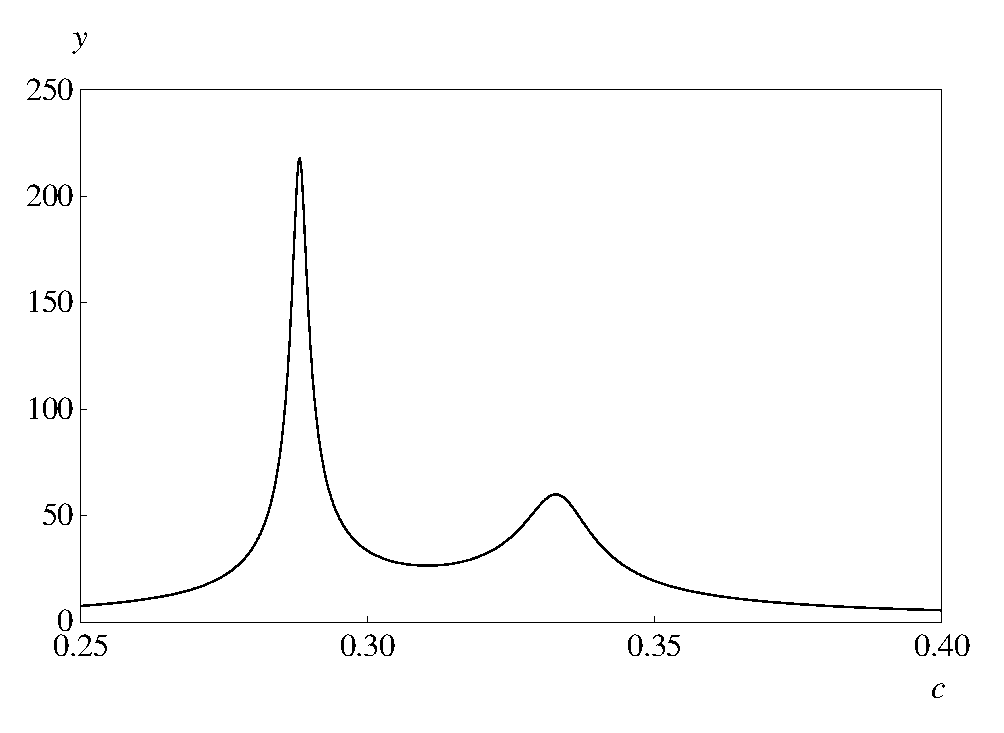
\includegraphics[width=0.95\textwidth]{images/Permit1.eps}
      \end{figure}
        \vspace{-10pt}\hfill
      \begin{minipage}[t]{0.9\textwidth}
        Залежність відносної дійсної частини ефективної проникності ($y = \varepsilon_{\rm eff}/\varepsilon_1$) від концентрації ядер $c$. 
        
        \vspace{5pt}
        Експериментальне підтверждення для ЖК систем: [S. Tomylko et al., Phys. Rev. E {\bf 92(1)} (2015) 012502]
      \end{minipage}
\end{columns}
\end{frame}

%%%%%%%%%%%%%%%%%%%%%%%%%%%%%%%%%%%%%%%%%%%%%%%%%%%%%
\begin{frame}{Ефективні критичні індекси перколяції}
\footnotesize

\vspace{-15pt}
\begin{columns}[T,onlytextwidth]
    \column{0.5\textwidth}
      \begin{figure}
        \centering
        $$x \sim (c-c_c)^t, \quad (c \to c_c+0)$$
        $$t_{\rm eff} = ln \frac{\sigma(c_2)}{\sigma(c_1)} / ln \frac{c_2-c_c}{c_1 - c_c}, \quad (c>c_c)$$
        \includegraphics[width=0.99\textwidth]{images/teff3.eps}
      \end{figure}
        Залежність ефективного індексу $t_{\rm eff}$ від $c_2$ при фіксованих $c_1$, $\delta=0.1$ ($c_c \approx 0.251$) та $x_2 = 5\times 10^{-5}$. Зверху вниз: $c_1 = 0.26, 0.27, 0.28$.\\
        Теорія перколяцій: $t \approx 1.3 \div 2.14$\\
        Експеримент: $t\approx 1.5 \div 2.0$ та вище

    \column{0.5\textwidth}
      \begin{figure}
        \centering
        $$x \sim (c_c-c)^{-s}, \quad (c \to c_c-0)$$
        $$s_{\rm eff} = - ln \frac{\sigma(c_2)}{\sigma(c_1)} / ln \frac{c_c-c_2}{c_c - c_1}, \quad (c<c_c)$$
        \includegraphics[width=0.99\textwidth]{images/seff3.eps}
      \end{figure}
      \hfill
      \begin{minipage}[t]{0.9\textwidth}
        Залежність ефективного індексу $s_{\rm eff}$ від $x_0 = \sigma_0/\sigma_1$ при  $\delta=0.1$ ($c_c \approx 0.251$), $x_2 = 5\times 10^{-5}$, $c_1 = 0.24$ та $c_2 = 0.25$.\\
        Теорія перколяцій: $s \approx 0.75$\\
        Експеримент: $s\approx 0.7 \div 1.0$
      \end{minipage}
\end{columns}

\end{frame}


%%%%%%%%%%%%%%%%%%%%%%%%%%%%%%%%%%%%%%%%%%%%%%%%%%%%%
\begin{frame}{Порівняння з експериментальними даними з проникності}

    \scriptsize{Експеримент: [D. Grannan, J. Garland, D. Tanner, Phys. Rev. Lett. {\bf 46} (1981) 375]}
    \footnotesize

\begin{columns}[T,onlytextwidth]
    \column{0.4\textwidth}
    \vspace{10pt}
      Еффективна проникність для двох зразків $\rm KCl-Ag$ (круги й трикутники) до порога перколяції та обробка згідно нашої теорії. 
      
      \vspace{5pt}
      -- Чорні лінії ($\circ$):\\
      $\varepsilon_0 = 5.0$, \\
      $\delta = 0.194$, \\
      $s = 0.72$. \\
      -- Сирі лінії ($\bigtriangleup$):\\
      $\varepsilon_0 = 7.0$, \\
      $\delta = 0.150$, \\
      $s = 0.74$.
      

    \column{0.6\textwidth}
      \begin{figure}
        \centering
        \includegraphics[width=0.99\textwidth]{images/KCl-Ag-eps.eps}
      \end{figure}
\end{columns}

\end{frame}
%}

%%%%%%%%%%%%%%%%%%%%%%%%%%%%%%%%%%%%%%%%%%%%%%%%%%%%%
\subsection{Порівняння з експериментальними даними}
%{\setbeamertemplate{frame footer}{Експеримент: [I.-G. Chen, W. Johnson, J. Mat. Sci. {\bf 21} (1986) 3162]}
\begin{frame}{Порівняння з експериментальними даними з провідності}

    \scriptsize{Експеримент: [I.-G. Chen, W. Johnson, J. Mat. Sci. {\bf 21} (1986) 3162]}
    
\footnotesize
\begin{columns}[T,onlytextwidth]
    \column{0.4\textwidth}
    \vspace{10pt}
      Ефективний питомий опір зразку композита $\rm KCl-Ag$ (квадрати) та обробка згідно нашої теорії: \\
      $\sigma_0 \approx 3.15 \times 10^{-8}$~См/м; \\
      $\sigma_1 \approx 6.25 \times 10^7$~См/м; 
      $\sigma_2 \approx 0.3 \times 10^3$~См/м; \\
      $\delta = 0.1682$ ($c_c = 0.214$).

      \vspace{5pt}
      Середній радіус частинок $\rm Ag$: $R\approx 10$~нм. 
      
      Вимірювана товщина оболонки: $\delta \approx 0.1$.

    \column{0.6\textwidth}
      \begin{figure}
        \centering
        \includegraphics[width=0.99\textwidth]{images/chen-grannan-s2-lin.eps}
      \end{figure}
\end{columns}

\end{frame}
%}
%{\setbeamertemplate{frame footer}{Експеримент: [D. Grannan, J. Garland, D. Tanner, Phys. Rev. Lett. {\bf 46} (1981) 375]}

%%%%%%%%%%%%%%%%%%%%%%%%%%%%%%%%%%%%%%%%%%%%%%%%%%%%%%%%%%%%%%%%%%%%%%%%%%%%%%%%%%%%%%%%%%%
\section{Застосування підходу до аналізу диференціального метода}%%%%%%%%%%%%%%%%%%%%%%%%%%%%%%%
%%%%%%%%%%%%%%%%%%%%%%%%%%%%%%%%%%%%%%%%%%%%%%%%%%%%%%%%%%%%%%%%%%%%%%%%%%%%%%%%%%%%%%%%%%

\begin{frame}{Диференціальний метод (асиметричний підхід Бругемана)}
\footnotesize

Розглянемо систему твердих діелектричних куль в діелектричній матриці при деякій концентрації $c$ та ефективній проникності $\varepsilon$.

Моделювання в рамках {\bf асиметричного підходу Бругемана (ABM)}:

\begin{wrapfigure}{r}{0.55\textwidth}
\vspace{-20pt}
  \begin{center}
    \begin{overpic}[width=0.55\textwidth]{images/hanai-fig1.eps}
         %\put(60,70){$\rm KCl/Ag$}
    \end{overpic}
  \end{center}
\vspace{-25pt}
\end{wrapfigure}
\textbf{Зміна~проникності~системи внаслідок~додавання інфінітезимальної~порції частинок~описується~як взаємодія цієї~порції~з існуючим ефективним середовищем в рамках моделі Максвелла-Гарнетта.}
$$
    \frac{\varepsilon - \varepsilon_0}{2\varepsilon_0 + \varepsilon} = c \frac{\varepsilon_1 - \varepsilon_0}{2\varepsilon_0 + \varepsilon_1}
$$

%Зазвичай застосовується для опису діелектричних властивостей емульсій, грунту, тощо.

Низькі $c$:\quad $\varepsilon_0 \to \varepsilon$;\quad $\varepsilon \to \varepsilon + \Delta\varepsilon$;\quad $c \to \Delta c/(1-c)$
\begin{equation}
     \frac{\Delta \varepsilon}{3\varepsilon} = \frac{\Delta c}{1-c} \frac{\varepsilon_1 - \varepsilon}{2\varepsilon + \varepsilon_1}  
    \quad \Rightarrow \quad
      1 - c = \frac{\varepsilon - \varepsilon_1}{\varepsilon_0 - \varepsilon_1} \left( \frac{{ \varepsilon_0}}{\varepsilon} \right)^{1/3}.
\end{equation}

Високі $c$:\quad $\varepsilon_0 \to \varepsilon_1$;\quad $\varepsilon_1 \to \varepsilon$;\quad $\varepsilon \to \varepsilon + \Delta\varepsilon$;\quad $c \to -\Delta c/c$
\begin{equation}
    \frac{\Delta \varepsilon}{3\varepsilon} = -\frac{\Delta c}{c} \frac{\varepsilon_0 - \varepsilon}{2\varepsilon + \varepsilon_0}  
    \quad \Rightarrow \quad
    c = \frac{\varepsilon - \varepsilon_0}{\varepsilon_1 + \varepsilon_0} \left( \frac{\varepsilon_1}{\varepsilon} \right)^{1/3}.
\end{equation}


\end{frame}
%%%%%%%%%%%%%%%%%%%%%%%%%%%%%%%%%%%%%%%%%%%%%%%%%%%%%
\begin{frame}{Побудова диференціальної схеми в рамках МКГ}
\footnotesize


Стара компактна група:
\begin{equation}\label{eq:delta-Brug}
\begin{split}
  {\delta\varepsilon}_{\rm CGA} ({\bf r}) = (\varepsilon_0 - \varepsilon) [1 - {\Pi}_1 ({\bf r})]+ (\varepsilon_1 - \varepsilon) [{\Pi}_1 ({\bf r})] 
\end{split}
\end{equation}

Нова компактна група:
\begin{equation}\label{eq:delta-Brug-diff0}
\begin{split}
  \widetilde{\delta\varepsilon}_{\rm CGA} ({\bf r}) =& (\varepsilon_0 - (\varepsilon + \Delta\varepsilon)) [1 - ({\Pi}_1 ({\bf r}) + \Delta{\Pi}_1 ({\bf r}))]\\
  &+ (\varepsilon_1 - (\varepsilon +   \Delta\varepsilon)) [{\Pi}_1 ({\bf r}) + \Delta{\Pi}_1 ({\bf r})] .
\end{split}
\end{equation}
Нехтуючи другими порядками малості за $\Delta\varepsilon$ та $\Delta c$:
\begin{equation}\label{eq:delta-Brug-diff}
\begin{split}
  \widetilde{\delta\varepsilon}_{\rm CGA} ({\bf r}) \approx \delta\varepsilon_{\rm CGA} ({\bf r})+ \delta\varepsilon_{\rm ABM}^{(l)} ({\bf r}) + \delta\varepsilon_{\rm ABM}^{(h)} ({\bf r}) ,
\end{split}
\end{equation}
%\begin{center}
\begin{tabular}{ ll } 
 $\delta\varepsilon_{\rm CGA} = (\varepsilon_0 - \varepsilon)[1 - \Pi_1] + (\varepsilon_1 - \varepsilon)\Pi_1$ & внесок заданої компактної групи;\\
 $\delta\varepsilon_{\rm ABM}^{(l)} = -\Delta\varepsilon [1 - \Pi_1] + (\varepsilon_1 - \varepsilon) \Delta\Pi_1$ & враховує вплив нових частинок на $\delta\varepsilon_{\rm CGA}$;\\
% & на проникність заданої компактної групи;\\ 
 $\delta\varepsilon_{\rm ABM}^{(h)} = -\Delta\varepsilon \Pi_1 - (\varepsilon_0 - \varepsilon)\Delta\Pi_1$ & враховує вплив зміни матриці на $\delta\varepsilon_{\rm CGA}$.
% & на проникність заданої компактної групи.
\end{tabular}
%\end{center}

\textbf{Класичні закони ABM отримаємо, якщо знехтувати внесками $\delta\varepsilon_{\rm CGA}$ та $\delta\varepsilon_{\rm ABM}^{(h)}$ (або $\delta\varepsilon_{\rm CGA}$ та $\delta\varepsilon_{\rm ABM}^{(l)}$). Це можливо лише за умов, що}\\
1) концентрація компоненту, що додається, мала; \\
2) різниці між діелектричними проникностями компонентів малі.

\end{frame}

%%%%%%%%%%%%%%%%%%%%%%%%%%%%%%%%%%%%%%%%%%%%%%%%%%%%%
\begin{frame}{Порівняння результатів з границями Хашина-Штрікмана}
\footnotesize
Узагальнення класичних правил ABM отримаємо, нехтуючи лише внеском $\delta\varepsilon_{\rm ABM}^{(h)}$ (або $\delta\varepsilon_{\rm ABM}^{(l)}$), але вони порушують класичні межі Хашина-Штрікмана. 
\begin{figure}[tb]
    \centering
    \includegraphics[width=0.55\textwidth]{images/hanai-fig2.eps}
    \caption{\label{fig:HSbounds}
    Концентраційна залежність $\varepsilon$ від $c$ (при $\varepsilon_1/\varepsilon_0 = 10^2$): а) узагальнення ABM в рамках МКГ (товсті чорні лінії 1, 2); б) межі Хашина-Штрікмана (тонкі лінії 3 та 4); в) МКГ (штрихована лінія); г) класичні правила ABM (точкові лінії 5 та 6).}
\end{figure}

\end{frame}


%%%%%%%%%%%%%%%%%%%%%%%%%%%%%%%%%%%%%%%%%%%
\section{Основні результати дослідження}%%%%%%%%%%%%%%%%%%%%%%%%%
%%%%%%%%%%%%%%%%%%%%%%%%%%%%%%%%%%%%%%%%%%%

\begin{frame}{Основні результати дослідження}
\footnotesize

1. Адекватний опис макроскопічних електричних властивостей реальних дисперсних систем вимагає виходу за межі двофазних моделей. Зокрема, він може ефективно здійснюватися в рамках статистичної моделі ефективного електричного відгуку невпорядкованих систем частинок з морфологією тверде ядро--проникна оболонка, побудованої в роботі шляхом узагальнення методу компактних груп на системи провідних частинок.

2. Отримані рівняння для ефективної статичної провідності розглянутих модельних систем підтверджуються результатами порівняння їх розв'язків з даними симуляцій, отриманих методом Random Resistor Network як для електрично однорідних, так і неоднорідних проникних оболонок. 

3. При відповідному виборі одночастинкових профілів провідності оболонок модель кількісно описує експериментальні дані для квазістатичної провідності різних типів твердих композитних та полімерних композитних електролітів. Ці профілі ефективно враховують вплив основних міжфазних та матричних фізико-хімічних механізмів в системі на формування її електричних властивостей та можуть бути використані для аналізу цих механізмів.

\end{frame}
%%%%%%%%%%%%%%%%%%%%%%%%%%%%%%%%%%%%%%%%%%%

\begin{frame}{Основні результати дослідження}
\footnotesize

4. Також модель кількісно описує поведінку ефективних провідності та діелектричної проникності твердих невпорядкованих композитів типу діелектрик--провідник з проникним міжфазним шаром. Положення порогу електричної перколяції в моделі визначається відносною товщиною оболонки, а значення ефективних критичних індексів для цих систем залежать як від геометричних та електричних параметрів компонентів, так і способу обробки експериментальних даних, а тому демонструють широкий спектр значень спостережуваних на експерименті.

5. Диференціальна схема аналізу ефективних квазістатичних електричних параметрів дисперсних систем є застосовною лише для систем з малими різницями діелектричних проникностей компонентів у вузьких концентраційних інтервалах диспергованих компонентів.

\end{frame}

%%%%%%%%%%%%%%%%%%%%%%%%%%%%%%%%%%%%%%%%%%%%%%%%%%%%%
{\setbeamercolor{palette primary}{fg=black, bg=white}
\begin{frame}[standout]
  Дякую за увагу!
\end{frame}
}

\appendix

%%%%%%%%%%%%%%%%%%%%%%%%%%%%%%%%%%%%%%%%%%%%%%%%%%%%%
\begin{frame}{Формалізм МКГ}
\footnotesize

[Сушко М.Я., ЖЭТФ {\bf 132} (2007) 478; J. Phys. D: Appl. Phys. {\bf 42} (2009) 155410; Phys. Rev. E {\bf 96} (2017) 062121]

\begin{list}{$\bullet$}{\leftmargin=1em \itemindent=0em}
\item
Розглядається рівняння розповсюдження електромагнітної хвилі в неоднорідному середовищі з розподілом проникності $\hat{\varepsilon}({\bf r}) = \hat{\varepsilon}_{\rm f} + \delta\hat{\varepsilon}({\bf r})$:
\begin{equation} \label{eq:propogate_eq}
\Delta {\bf E} ({\bf r}) - {\rm grad}\, {\rm div} {\bf E} ({\bf r}) + k_0^{2}\hat{\varepsilon}_{\rm f} {\bf E} ({\bf r})  = - k_{0}^{2} \delta
\hat{\varepsilon} ({\bf r}) {\bf E} ({\bf r}).
\end{equation}

\item 
Еквівалентне інтегральне представлення:
\begin{equation}\label{eq:integral_field}
{\bf E}({\rm {\bf r}}) = {\bf E}_{0} ({\bf r}) -
k_{0}^{2} \int\limits_{V} d{\bf r}'\, {\rm T}(|{\bf r} - {\bf r}'|)
\delta \hat{\varepsilon} ({\bf r}')\, {\bf E}({\bf r}').
\end{equation}

\item 
Рішення шукається ітераційним методом:
\begin{equation}\label{eq:iterationE}
{\bf E} ({\bf r}) = {\bf E}_0 ({\bf r}) +
\sum\limits_{s=1}^{\infty} {\bf E}_s ({\bf r}),
\end{equation}
\begin{equation*}
\begin{split}
{\bf E}_s ({\bf r}) =& (- k_0)^{2s} \int\limits_V d{\bf r_1}
\int\limits_V d{\bf r}_2 \,...\, \int\limits_V d{\bf r}_s
{\rm T}(|{\bf r} - {\bf r}_1|) {\rm T}(|{\bf r}_1 - {\bf r}_2|)
\,...\, {\rm T}(|{\bf r}_{s-1} - {\bf r}_s|) \times \\
&\times \delta{\varepsilon} ({\bf r}_1) \delta{\varepsilon} ({\bf r}_2)
\,...\, \delta{\varepsilon} ({\bf r}_s) {\bf E}_0 ({\bf r}_s).
\end{split}
\end{equation*}

\end{list}

\end{frame}

%%%%%%%%%%%%%%%%%%%%%%%%%%%%%%%%%%%%%%%%%%%%%%%%%%%%%
\begin{frame}{Представлення пропагатора та результат для $\langle {\bf E} \rangle$ та $\langle {\bf J} \rangle$}
\footnotesize

\begin{list}{$\bullet$}{\leftmargin=1em \itemindent=0em}
\item
Компоненти пропагатора $\rm T$:
$$
    T_{\alpha\beta} = -(k^2 \delta_{\alpha\beta + \nabla_\alpha\nabla_\beta}) \frac{e^{ikr}}{4\pi k^2 r}
$$
розкладаються на сингулярну та головну частини [Weiglhofer W., Am. J. Phys. {\bf 57} (1989) 455]:
\begin{equation}\label{eq:propagator-CGA}
\begin{split}
{\widetilde T}_{\alpha\beta} &({\rm {\bf r}})
= {\widetilde T}_{\alpha\beta}^{(1)} ({\rm {\bf r}}) +
{\widetilde T}_{\alpha\beta}^{(2)} ({\rm {\bf r}}) +
{\widetilde T}_{\alpha\beta}^{(3)} ({\rm {\bf r}})
= \frac{1}{3k^{2}} \delta_{\alpha\beta} \delta ({\rm
	{\bf r}})\,e^{ikr} + \\
&+ \frac{1}{4\pi k^{2}}
\left(\frac{1}{r^3}-\frac{ik}{r^2}\right)
\left( \delta _{\alpha\beta} - 3e_{\alpha} e_{\beta}
\right)\,e^{ikr} - \frac{1}{4\pi r}\left( {\delta
	_{\alpha\beta} - e_{\alpha} e_{\beta}} \right)\,e^{ikr},
\end{split}
\end{equation}
вважаючи, що для достатньо добрих функцій $\psi({\bf r})$ виконується
$$
    \int\limits_V {\rm T}(r) \psi({\bf r}) d{\bf r} = \int\limits_V {\widetilde{\rm T}}(r) \psi({\bf r}) d{\bf r}.
$$

\item
Основний результат для $\langle {\bf E} \rangle$ та $\langle {\bf J} \rangle$:
\begin{equation}\label{eq:E_average-J_average}
\langle {\bf E} ({\bf r}) \rangle = \left[ 1 + \langle \hat{Q}({\bf r}) \rangle \right] {\bf E}_0;
\qquad 
\langle {\bf J} ({\bf r}) \rangle = - i \frac{\omega\hat{\varepsilon}_{\rm f}}{4\pi} \left[ 1 - 2\langle \hat{Q}({\bf r}) \rangle \right] {\bf E}_0,
\end{equation}
де
\begin{equation}\label{eq:Q-sum}
\hat{Q}({\bf r}) = \sum\limits_{s=1}^{\infty} \left( - \frac{1}{3\hat{\varepsilon}_{\rm f}} \right)^s (\delta\hat{\varepsilon}({\bf r}))^s.
\end{equation}

Було знехтувано вкладами порядку $|\hat{\varepsilon}_{\rm f}|k_0^2 L^3/d$ при переході $\sqrt{|\hat{\varepsilon}_{\rm f}|}k_0 \to 0$ ($L/d \sim 1$ для кінцевих $L$).

\end{list}

\end{frame}


%%%%%%%%%%%%%%%%%%%%%%%%%%%%%%%%%%%%%%%%%%%%%%%%%%%%%
\begin{frame}{Збіжність $\hat{Q}({\bf r})$}
\footnotesize

\begin{list}{$\bullet$}{\leftmargin=1em \itemindent=0em}
\item
Перейдемо до наближення $\omega \to 0$ одразу на етапі розкладу пропагатора:
\begin{equation}\label{eq:prop_longwave}
	\lim\limits_{\omega \to 0} \hat{\varepsilon}_{\rm f} k_0^2  \widetilde{T}_{\alpha\beta} = \tau_{\alpha\beta}^{(1)} + \tau_{\alpha\beta}^{(2)} =
	\frac{1}{3} \delta({\bf r}) \delta_{\alpha\beta} + \frac{\delta_{\alpha\beta} - 3e_\alpha e_\beta}{4\pi r^3}.
\end{equation}

\item
Отримаємо для $\langle {\bf E} \rangle$ та $\langle {\bf J} \rangle$:
\begin{equation}\label{eq:E-averaged-direct}
\langle {\bf E}({\bf r}) \rangle = 
\left[ 1 + \langle \hat{Q}({\bf r}) \rangle \right] {\bf E}_0 
- 3 \int\limits_V d{\bf r}' \tau^{(2)} (|{\bf r} - {\bf r}'|) \left\langle \frac{\delta\hat{\varepsilon}({\bf r}')}{3\hat{\varepsilon}_{\rm f} + \delta\hat{\varepsilon}({\bf r})} {\bf E}({\bf r}') \right\rangle ,
\end{equation}
\begin{equation}\label{eq:C-averaged-direct}
\begin{split}
\langle {\bf J}({\bf r}) \rangle =& 
- i \frac{\omega}{4\pi} \hat{\varepsilon}_{\rm f} \left[ 1 - 2\langle \hat{Q}({\bf r}) \rangle \right] {\bf E}_0 \\
&+ i \frac{3}{4\pi} \int\limits_V d{\bf r}' \tau^{(2)} (|{\bf r} - {\bf r}'|) \left\langle \frac{\omega \hat{\varepsilon}({\bf r}) \delta\hat{\varepsilon}({\bf r}')}{3\hat{\varepsilon}_{\rm f} + \delta\hat{\varepsilon}({\bf r})} {\bf E}({\bf r}') \right\rangle.
\end{split}
\end{equation}
де
\begin{equation}\label{eq:Q}
\hat{Q}({\bf r}) = -\frac{\delta\hat{\varepsilon} ({\bf r})}{3\hat{\varepsilon}_{\rm f} + \delta\hat{\varepsilon}({\bf r})}.
\end{equation}

Для макроскопічно однорідних та ізотропних систем статистичні середні залежать лише від $|{\bf r} - {\bf r}'|$, тому внески від $\tau^{(2)}$ зануляються.

\end{list}

\end{frame}

%%%%%%%%%%%%%%%%%%%%%%%%%%%%%%%%%%%%%%%%%%%%%%%%%%%%%
\begin{frame}{Використані параметри: обробка даних симуляцій RRN}
\footnotesize

\begin{table}[bt]
	\begin{center}%\centering
		\caption{\label{tab:RRN-exper-params} Значення провідності відповідних компонент системи в С/см, що використовувались в числових експериментах RRN.}\vspace{-10pt}
		\begin{tabular}{|l|c|c|c|c|c|}
			\hline
			Моделі оболонки  & $\sigma_0$ & $\sigma_1$ & $\sigma_2$ & $\sigma_{\rm min}^\prime$ & $\sigma_{\rm max}^\prime$ \\
			\hline
			однорідна  & $1\times 10^{-8}$ & $1\times 10^{-12}$ & $1\times 10^{-4}$     & & \\
			\hline
			неоднорідна  & $1\times 10^{-8}$ & $1\times 10^{-12}$ &   & $1\times 10^{-6}$ & $1\times 10^{-4}$\\
			\hline
		\end{tabular}
	\end{center}
\end{table}

\begin{table}[htb]
	\centering
	\caption{Використані параметри для обробки даних симуляцій для однорідних та неоднорідних оболонок, відповідно.}\vspace{-10pt}
	\label{tab:numerical-homogeneous}
	\begin{tabular}{|l|l|r|r|r|r|r|}
		\hline
		\multirow{2}{*}{(а)} & $d$, мкм & 3 & 5 & 7 & 9 & 11 \\ \cline{2-7} 
		& $K/k$ & 1.0 & 1.05 & 1.05 & 1.07 & 1.10 \\ \hline
		\multirow{2}{*}{(б)} & $t$, мкм & 3 & 5 & 7 & 9 & 11 \\ \cline{2-7} 
		& $K/k$ & 1.08 & 1.05 & 1.06 & 1.07 & 1.06 \\ \hline
	\end{tabular}
	
		\begin{tabular}{|l|l|r|r|r|r|r|}
			\hline
			\multirow{3}{*}{(а)} & $d$, мкм & 3    & 5    & 7     & 9     & 11    \\ \cline{2-7}
			& $K/k$    & 1.09 & 1.02 & 1.13  & 1.11  & 1.09   \\ 
			\cline{2-7}
			& ${\rm log_{10}}\left(\sigma_{\rm max}/\sigma_{\rm min}\right)$
			& 1.83 & 1.89 & 1.82 & 1.88 & 1.98\\
			\hline
			\multirow{3}{*}{(б)} & $t$, мкм & 3    & 5    & 7     & 9     & 11    \\ \cline{2-7}
			& $K/k$    & 1.00  & 1.00  & 1.05 & 1.07 & 1.13  \\ \cline{2-7}
			& ${\rm log_{10}}\left(\sigma_{\rm max}/\sigma_{\rm min}\right)$
			& 1.90  & 1.89  & 1.85 & 1.85 & 1.87 \\
			\hline
		\end{tabular}
\end{table}

\end{frame}

%%%%%%%%%%%%%%%%%%%%%%%%%%%%%%%%%%%%%%%%%%%%%%%%%%%%%
\begin{frame}{Використані параметри: обробка даних ТКЕ при 25$\rm ^{o}C$}
\footnotesize

\begin{table}[tb]
	\caption{\label{tab:Liang} Параметри, що використовувались для обробки
		даних з $\sigma_{\rm eff}$ для ТКЕ $\rm{LiI/Al_2O_3}$
		в рамках а) однорідної, б) подвійної та в) сигмойдної 
		моделей профілів $\sigma_2(r)$;
		$\sigma_0 = 2.5 \times 10^{-7}\,{\rm S/cm}$,  $x_1 = 0$.}
	\begin{center}
		\begin{tabular}{|l|l|l|l|l|l|}
			\hline
			а) & $x_2$ & $\delta$ & &  &  \\
			& 150    & 0.5   &  &  & \\
			\hline
			б)  & $x_{2,1}$   &$x_{2,2}$ & $\delta_1$ & $\delta_2$ &  \\
			& 185         & 14  & 0.40       & 1.50       &  \\
			\hline
			в)  & $x^{\ast}_{2,1}$    &$x^{\ast}_{2,2}$    & $\delta^{\ast}_1$ & $\delta^{\ast}_2$ &  $\alpha$ \\
			& 185         & 12        & 0.38       & 1.41       &   0.03    \\
			\hline
		\end{tabular}
	\end{center}
\end{table}

\end{frame}


%%%%%%%%%%%%%%%%%%%%%%%%%%%%%%%%%%%%%%%%%%%%%%%%%%%%%
\begin{frame}{Використані параметри: обробка даних ПКЕ при 25$\rm ^{o}C$}
\footnotesize

\begin{table}[tb]
	\centering 
	\caption{\label{tab:adjustable_params-1} Параметри, що
		використані для обробки даних з 
		концентраційних залежностей $\sigma_{\rm eff}$ ПКЕ в 
		рамках моделей однорідної, двошарової
		та неперервних оболонок.}
	\vspace{-10pt}
	\begin{threeparttable}
		\begin{tabular}{|l|l|l|l|l|l|l|l|}
			\hline
			\multirow{2}{*}{Оболонка} &\multirow{2}{*}{L\tnote{a}} &   \multirow{2}{*}{$x_1$} & $\delta_1$\tnote{b} & $\delta_2$\tnote{b}  & $x_{21}$\tnote{b} & $x_{22}$\tnote{b} &  \multirow{2}{*}{$R^2$, \%} \\
			&  & & $\delta^\ast_1$\tnote{c}& $\delta^\ast_2$\tnote{c}&$x^\ast_{21}\tnote{c}$&$x^\ast_{22}$\tnote{c} & \\
			\hline
			\multicolumn{8}{c}{PEO--NaI--NASICON ($\sigma_0 \approx 9.86\times 10^{-9}$~S/cm)}\\
			\hline
			однорідна  &1a   & $1.4\times 10^4$ &1.6& -- &  1000& -- & --  \\
			однорідна                 &1b                                       &1.4             &1.6& -- &  1300& -- & --  \\
			подвійна                 &1c                                       &70              &1.0&1.55&  400  &  20000 &  99.4 \\
			неперервна, &1d                   &70              &1.0&1.55&  400 &  6000 &  95.5 \\
			$\alpha =0.05$   & & & & & &  &   \\
			\hline
			\multicolumn{8}{c}{(PEO)$_{10}$--NaI--$\theta$-Al$_2$O$_3$ ($\sigma_0 \approx 1.54\times 10^{-8}$~S/cm)}\\
			\hline
			однорідна &2a & \multirow{5}{*}{$6.5\times 10^{-13}$} &2.1&--&230&--&--  \\
			подвійна &2b                                       &                   &0.7&2.1&0.12&435& 92.8\\
			подвійна &2c                                       &                   &0.8&2.1&0.12&520& 98.6\\
			неперервна, &2d                                  &                   &0.9&2.1&0.12&560& 95.0\\
			$\alpha =0.05$  &  &  & & & &  &   \\
			\hline
		\end{tabular}
		\begin{tablenotes}
			\item[a] Використані позначення для підгонок на відповідних
			рисунках.
			\item[b] Параметри для моделей ступінчатих оболонок.
			\item[c] Параметри для моделей неперервних оболонок.
		\end{tablenotes}
	\end{threeparttable}
\end{table}

\end{frame}


%%%%%%%%%%%%%%%%%%%%%%%%%%%%%%%%%%%%%%%%%%%%%%%%%%%%%
\begin{frame}{Використані параметри: обробка даних ПКЕ при 25$\rm ^{o}C$}
\footnotesize

\begin{table}[tb]
	\centering 
	\caption{\label{tab:adjustable_params-2} Параметри, що
		використані для обробки даних з 
		концентраційних залежностей $\sigma_{\rm eff}$ ПКЕ в 
		рамках моделей двошарової, тришарової
		та неперервних оболонок.}
	\vspace{-5pt}
	\begin{threeparttable}
		\begin{tabular}{|l|l|l|l|l|l|l|l|l|}
			\hline
			\multirow{2}{*}{Оболонка} &\multirow{2}{*}{L\tnote{a}} & $\delta_1$\tnote{b} & $\delta_2$\tnote{b} & $\delta_3$\tnote{b} & $x_{21}$\tnote{b} & $x_{22}$\tnote{b} & $x_{23}$\tnote{b} & \multirow{2}{*}{$R^2$, \%} \\
			&  & $\delta^\ast_1$\tnote{c}& $\delta^\ast_2$\tnote{c}&$\delta^\ast_3$\tnote{c}&$x^\ast_{21}\tnote{c}$&$x^\ast_{22}$\tnote{c}&$x^\ast_{23} \tnote{c}$ & \\
			\hline
			\multicolumn{9}{c}{PEO--LiClO$_4$--PAAM ($\sigma_0 \approx 6.12\times 10^{-7}$~S/cm; $x_1 \approx 1.6 \times 10^{-6}$)}\\
			\hline
			подвійна &3a & 0.15&0.60& -- & 5.0           &800 &--& 88.7 \\
			потрійна  &3b              &0.16&0.50&0.80 & 5.0 &1800 &27 &  92.3 \\
			неперервна,  &3c                      &  0.32&0.45&0.48 & 2.0     &9400&27 & 92.9 \\
			$\alpha =0.03$ &   & & & & &  & & \\
			\hline
			\multicolumn{9}{c}{OMPEO--LiClO$_4$--PAAM, після отжигу ($\sigma_0 \approx 1.61\times 10^{-5}$~S/cm; $x_1 \approx 6.2\times 10^{-8}$)}\\
			\hline
			подвійна   &4a   &0.36&0.75& -- &0.60& 75 &--& 46.3\\
			потрійна   & 4b             &0.40&0.80&1.40&0.57& 750&0.10 &  93.8\\
			неперервна, &4c       &0.54&0.64&1.53&0.44&14200&0.10 &  81.7\\
			$\alpha =0.02$ &  &  & & & &  & & \\
			\hline
		\end{tabular}
		\begin{tablenotes}
			\item[a] Використані позначення для підгонок на відповідних
			рисунках.
			\item[b] Параметри для моделей ступінчатих оболонок.
			\item[c] Параметри для моделей неперервних оболонок.
		\end{tablenotes}
	\end{threeparttable}
\end{table}

\end{frame}


%%%%%%%%%%%%%%%%%%%%%%%%%%%%%%%%%%%%%%%%%%%%%%%%%%%%%
\begin{frame}{Використані параметри: обробка ізотерм ПКЕ}
\footnotesize

\begin{table}[tb]
	\centering
	\begin{threeparttable}
		\caption{\label{tab:isotherms} Значення провідності, в См/см, що були використані для підгонок ізотерм концентраційних залежностей $\sigma_{\rm{eff}}$ для ПКЕ OMPEO--LiClO$_4$--PAAM \tnote{a,b}. }
		
		\begin{tabular}{|l|l|l|l|}
			\hline
			{Складова}   & $t = 0\,\rm { ^oC}$ & $t = 25\, \rm {^oC}$ & $t = 100\, \rm {^oC}$ \\
			\hline
			Матриця, $\sigma_0$           &  $4.64\times 10^{-7}$  &  $1.57\times 10^{-5}$  &  $1.78\times 10^{-3}$   \\
			Перша оболонка, $\sigma_{21}$   &  $5.75\times 10^{-7}$  &  $8.70\times 10^{-6}$  &  $4.21\times 10^{-4}$    \\
			Друга оболонка, $\sigma_{22}$  &  $1.025\times 10^{-3}$ &  $7.74\times 10^{-3}$  &  $1.00\times 10^{-1}$   \\
			Третя оболонка, $\sigma_{23}$   &  $1.07\times 10^{-7}$  &  $3.12\times 10^{-6}$  &  $1.36\times 10^{-4}$ \\
			\hline
		\end{tabular}
		\begin{tablenotes}
			\item[a] З молярною долею LiClO$_4$ 10 \%. 
			\item[b] За рахунок формування комплексів катіонів $\rm{Li}^+ $
			з ланцюгами PAAM, ядра PAAM--LiClO$_4$ непровідні, та мають
			при кімнатній температурі провідність 
			$\sigma_1\sim 1\times 10^{-12}$~См/см. 
			Це значення й було використано в наших розрахунках.
			Зростання $\sigma_1$ на декілька порядків не вплинуло
			на отримані результати (у границях потрібної точності).
		\end{tablenotes}
	\end{threeparttable}
\end{table}

\end{frame}


%%%%%%%%%%%%%%%%%%%%%%%%%%%%%%%%%%%%%%%%%%%%%%%%%%%%%
\begin{frame}{Використані параметри: обробка ізохор ПКЕ}
\footnotesize

\begin{table}[tb]
	\centering
	\begin{threeparttable} 
	\caption{\label{tab:temp} Параметри VTF, що отримані для ПКЕ OMPEO--LiClO$_4$--PAAM \tnote{a}}
		\begin{tabular}{|l|l|l|l|}
			\hline
			{Складова}   & $A$, См$\cdot \rm{K}^{1/2}/$см & $B$, K & $T_0$, K  \\
			\hline
			Матриця, $\sigma_0$           &  36.1\tnote{a}  &  1270  &  190   \\
			Перша оболонка, $\sigma_{21}$   &  4.33  &  1210   &  180    \\
			Друга оболонка, $\sigma_{22}$  &  71.1   &  634     &  197   \\
			Третя оболонка, $\sigma_{23}$   & 0.229   &  720   &  212 \\
			\hline
		\end{tabular}
		\begin{tablenotes}
			\item[a] З молярною долею LiClO$_4$ 10 \%.
		\end{tablenotes}
	\end{threeparttable}
\end{table}

\end{frame}

\end{document}
